\emph{La pièce est équilibrée : $P(A) = P(B) = 0,5$. On a $P_A(D) = 0,6$ et $P_B\left(\overline{D}\right) = 0,8$.}

\begin{enumerate}
	\item La somme des probabilités issues d'un même n{\oe}ud vaut 1 :
	$P_A\left(\overline{D}\right) = 1 - 0,6 = 0,4$ et $P_B(D) = 1 - 0,8 = 0,2$.

	\begin{center}
		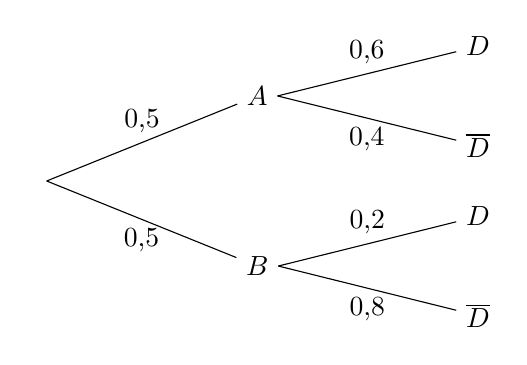
\begin{tikzpicture}[x=2.8cm, y=0.9cm]
			
			\node (root) at (0,0) {};
			\node (A) at (1,1.2) {$A$};
			\node (B) at (1,-1.2) {$B$};
			\node (D1) at (2,1.9) {$D$};
			\node (D1b) at (2,0.5) {$\overline{D}$};
			\node (D2) at (2,-0.5) {$D$};
			\node (D2b) at (2,-1.9) {$\overline{D}$};
			
			\draw (root.east) -- (A) node[pos=0.5,above] {0,5};
			\draw (root.east) -- (B) node[pos=0.5,below] {0,5};
			
			\draw (A.east) -- (D1) node[pos=0.5,above] {0,6};
			\draw (A.east) -- (D1b) node[pos=0.5,below] {0,4};
			\draw (B.east) -- (D2) node[pos=0.5,above] {0,2};
			\draw (B.east) -- (D2b) node[pos=0.5,below] {0,8};
		\end{tikzpicture}
	\end{center}

	\item $P(A \cap D) = P(A) \times P_A(D) = 0,5 \times 0,6 = 0,3$.

	La probabilité que le joueur pioche dans l'urne A et tire un jeton doré est égale à $0,3$.

	\item $A$ et $B$ forment une partition de l'univers. D'après la formule des probabilités totales :
	\[P(D) = P(A \cap D) + P(B \cap D) \]
	\[P(D) = P(A)\times P_A(D) + P(B)\times P_B(D) \]
	\[ P(D) = 0,5 \times 0,6 + 0,5 \times 0,2 = 0,3 + 0,1 = 0,4.\]

	\item On cherche $P_D(B)$. On a $P(B \cap D) = P(B) \times P_B(D) = 0,5 \times 0,2 = 0,1$, donc
	\[P_D(B) = \dfrac{P(B \cap D)}{P(D)} = \dfrac{0,1}{0,4} = 0,25.\]
	Sachant que le jeton obtenu est doré, la probabilité qu'il ait été pioché dans l'urne B
	est égale à $0,25$.
\end{enumerate}
